%%
%% Copyright 2007, 2008, 2009 Elsevier Ltd
%%
%% This file is part of the 'Elsarticle Bundle'.
%% ---------------------------------------------
%%
%% It may be distributed under the conditions of the LaTeX Project Public
%% License, either version 1.2 of this license or (at your option) any
%% later version.  The latest version of this license is in
%%    http://www.latex-project.org/lppl.txt
%% and version 1.2 or later is part of all distributions of LaTeX
%% version 1999/12/01 or later.
%%
%% This template has been modified by Philip Blakely for
%% local distribution to students on the MPhil for Scientific
%% Computing course run at the University of Cambridge.
%%

%% Template article for Elsevier's document class `elsarticle'
%% with numbered style bibliographic references
%% SP 2008/03/01
%%
%%
%%
%% $Id: elsarticle-template-num.tex 4 2009-10-24 08:22:58Z rishi $
%%
%%
\documentclass[final,3p,times,twocolumn]{elsarticle}

%% Use the option review to obtain double line spacing
%% \documentclass[preprint,review,12pt]{elsarticle}

%% Use the options 1p,twocolumn; 3p; 3p,twocolumn; 5p; or 5p,twocolumn
%% for a journal layout:
%% \documentclass[final,1p,times]{elsarticle}
%% \documentclass[final,1p,times,twocolumn]{elsarticle}
%% \documentclass[final,3p,times]{elsarticle}
%% \documentclass[final,3p,times,twocolumn]{elsarticle}
%% \documentclass[final,5p,times]{elsarticle}
%% \documentclass[final,5p,times,twocolumn]{elsarticle}

%% if you use PostScript figures in your article
%% use the graphics package for simple commands
%% \usepackage{graphics}
%% or use the graphicx package for more complicated commands
%% \usepackage{graphicx}
%% or use the epsfig package if you prefer to use the old commands
%% \usepackage{epsfig}

%% The amssymb package provides various useful mathematical symbols
\usepackage{amssymb}
%% The amsthm package provides extended theorem environments
%% \usepackage{amsthm}

%% The lineno packages adds line numbers. Start line numbering with
%% \begin{linenumbers}, end it with \end{linenumbers}. Or switch it on
%% for the whole article with \linenumbers after \end{frontmatter}.
%% \usepackage{lineno}

%% natbib.sty is loaded by default. However, natbib options can be
%% provided with \biboptions{...} command. Following options are
%% valid:

%%   round  -  round parentheses are used (default)
%%   square -  square brackets are used   [option]
%%   curly  -  curly braces are used      {option}
%%   angle  -  angle brackets are used    <option>
%%   semicolon  -  multiple citations separated by semi-colon
%%   colon  - same as semicolon, an earlier confusion
%%   comma  -  separated by comma
%%   numbers-  selects numerical citations
%%   super  -  numerical citations as superscripts
%%   sort   -  sorts multiple citations according to order in ref. list
%%   sort&compress   -  like sort, but also compresses numerical citations
%%   compress - compresses without sorting
%%
%% \biboptions{comma,round}

% \biboptions{}


\journal{MPhil in Scientific Computing}

\begin{document}

\begin{frontmatter}

%% Title, authors and addresses

%% use the tnoteref command within \title for footnotes;
%% use the tnotetext command for the associated footnote;
%% use the fnref command within \author or \address for footnotes;
%% use the fntext command for the associated footnote;
%% use the corref command within \author for corresponding author footnotes;
%% use the cortext command for the associated footnote;
%% use the ead command for the email address,
%% and the form \ead[url] for the home page:
%%
%% \title{Title\tnoteref{label1}}
%% \tnotetext[label1]{}
%% \author{Name\corref{cor1}\fnref{label2}}
%% \ead{email address}
%% \ead[url]{home page}
%% \fntext[label2]{}
%% \cortext[cor1]{}
%% \address{Address\fnref{label3}}
%% \fntext[label3]{}

\title{On the uses of \LaTeX}

%% use optional labels to link authors explicitly to addresses:
%% \author[label1,label2]{<author name>}
%% \address[label1]{<address>}
%% \address[label2]{<address>}

\author{Philip Blakely}

\address{Cavendish Laboratory, Department of Physics, J J Thomson
  Avenue, Cambridge. CB3 0HE}

\begin{abstract}
This is my abstract. This document is a demonstration of the power of
\LaTeX{} as originally developed by Leslie Lamport. We describe the
various features of \LaTeX{}, demonstrate the inclusion of elements such
as pictures, formul\ae, and references.
We conclude that LaTeX is a suitable system for producing professional
papers for publication in high-impact journals.
\end{abstract}

\end{frontmatter}

%%
%% Start line numbering here if you want
%%
% \linenumbers

%% main text
\section{\LaTeX{} features}
\LaTeX{} was originally developed by Leslie Lamport \cite{LaTeXBook} as a set of
macros on top of the \TeX{} language developed by Donald Knuth \cite{TeXBook}. It has a
number of features which make it well suited to professional
scientific publishing, including the ability to typeset mathematical
formul\ae, justify text well, and include pictures at various
points.\par
In section \ref{sect:Formulae} we show some mathematical formul\ae
that can be used within \LaTeX{}. In section \ref{sect:Pictures} we
demonstrate the inclusion of figures, including captions. Finally, in
\ref{sect:Concl}, we conclude that \LaTeX{} is an excellent typesetting
mechanism for scientific publications.

\section{Mathematical formulae}
\label{sect:Formulae}
Complex formulae are easy to produce within \LaTeX{}. For example, we
can use inline equations to define $f(x) = a_3x^3 + a_2x^2 + a_1x +
a_0$, and then provide more complex equations such as
\begin{equation}
\int_0^3 f(x) \mathrm{d}x = \left[\frac{a_3}{4}x^4 + \frac{a_2}{3}x^3
  + \frac{a_1}{2}x^2 + a_0x\right]_0^3
\label{eqn:Taylor}
\end{equation}
If we have some derivation that should belong elsewhere, we can put it
in an appendix such as \ref{app:quad}. We can also refer to equations
from the main text such as the Taylor expansion (\ref{eqn:Taylor}).
\section{Pictures}
\label{sect:Pictures}
In this section we demonstrate the inclusion of figures. For example,
Figure~\ref{fig:ENO1} demonstrates ENO as used to solve a linear advection
of a top-hat function.
\begin{figure}
\centering
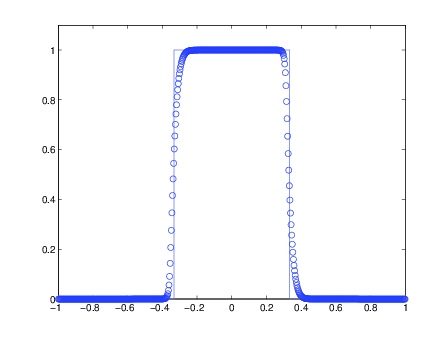
\includegraphics[width=3in]{ENOTest3b.png}
\caption{Demonstration of ENO as used to solver linear-advection of a
  top-hat function.}
\label{fig:ENO1}
\end{figure}
\section{Conclusions}
\label{sect:Concl}
In which we conclude that LaTeX (or \LaTeX) is very useful for
generating scientific papers as demonstrated above.

\section*{Acknowledgements}
Here I acknowledge the assistance of my supervisor, my industrial sponsor,
and the effects of caffeine on my ability to produce this report on time.

%% The Appendices part is started with the command \appendix;
%% appendix sections are then done as normal sections
\appendix

\section{On the Derivation of the Quadratic Formula}
\label{app:quad}
The derivation of the quadratic formula is something that would not
fit well within a paper as it would interrupt the flow of the argument
therein. However, for those students who need a refresher on how the
quadratic formula is derived, we give full details here:\par
Assume that we have
\begin{equation}
p(x) = ax^2 + bx + c
\end{equation}
and so on. The actual algebra is left as an exercise for the reader.

%% References
%%
%% Following citation commands can be used in the body text:
%% Usage of \cite is as follows:
%%   \cite{key}         ==>>  [#]
%%   \cite[chap. 2]{key} ==>> [#, chap. 2]
%%

%% References with bibTeX database:

\bibliographystyle{elsarticle-num}
\bibliography{references.bib}

%% Authors are advised to submit their bibtex database files. They are
%% requested to list a bibtex style file in the manuscript if they do
%% not want to use elsarticle-num.bst.

%% References without bibTeX database:

% \begin{thebibliography}{00}

%% \bibitem must have the following form:
%%   \bibitem{key}...
%%

% \bibitem{}

% \end{thebibliography}


\end{document}

%%
%% End of file `elsarticle-template-num.tex'.
